\section{Preliminaries}
\label{preliminary}

In our problem, we consider an undirected, unweighted graph $G = (V,E)$. The number of vertices is denoted as $n = |V|$ and number of edges is denoted as $m = |E|$. If the graph is weighted, we use $w_u$ and $w_e$ to denote the weight of vertex $u$ and edge $e$. We define the set of neighbors of a vertex $v$ in $G$ as $N_v = {u \in V :(v, u) \in E}$, and the degree of $v$ as $d_v = |N_v|$. We define a triangle in $G$ as a cycle of length 3. Let $u, v, w \in V$ be the three vertices on the cycle, and we denote this triangle by $\triangle_{uvw}$. Then we define several key concepts in this paper as follows.

\begin{Def}[Edge support]
The support of an edge $e_{u,v} \in E$ is defined as $s_{e,G} = |{\triangle_{uvw} : w \in V}|$. We denote it as $s_e$ when the context is clear.
\label{def:edge_support}
\end{Def}

\begin{Def}[Trussness] 
The trussness of a subgraph $H \in G$ is the minimum support of edges in $H$ plus $2$, denoted by $\tau_{H} = min\{(s_{e,H} + 2): e \in E_{H}\} $.  The trussness of an edge $e$ is defined as: $\tau_{e} = max_{H \in G}\{\tau_{H}: e \in E_{H}\}$.
\label{def:trussness}
\end{Def}

\begin{Def}[K-truss subgraph]
Given a graph $G$ and $k \ge 2$, $H \subseteq G$ is a k-truss if $\forall e \in E_{H}, s_{e,H} \ge (k - 2)$. 
\label{def:k-truss}
\end{Def}

\begin{Def}[Maximal k-truss subgraph]
$H$ is a maximal k-truss subgraph if it is not a subgraph of another k-truss subgraph with same trussness $k$ in $G$.
\label{def:maximal_k-truss}
\end{Def}

We use the same triangle adjacency and triangle connectivity definition as in~\cite{huang2014querying} listed below.

\begin{Def}[Triangle adjacency]
${\triangle}_{1}$, ${\triangle}_{2}$ are adjacent if they share a common edge, i.e., ${\triangle}_{1} \cap {\triangle}_{2} \neq \emptyset$. 
\label{def:triangle_adjacency}
\end{Def}

\begin{Def}[Triangle connectivity] 
${\triangle}_{1}$, ${\triangle}_{2}$ are triangle connected if they can reach each other through a series of adjacent triangles, \ie for $1 \le i < n, {\triangle}_{i} \cap {\triangle}_{i+1} \neq \emptyset$. 
\label{def:triangle_connectivity}
\end{Def}

\begin{Def}[Triangle connected graph]
Two edge $e_{1}, e_{2}$ are triangle connected in a subgraph $H$ if there are two triangle ${\triangle}_{1}, {\triangle}_{2}$ in $H$ and $e_{1} \in {\triangle}_{1}, e_{2} \in {\triangle}_{2}$, either ${\triangle}_{1} = {\triangle}_{2}$, or ${\triangle}_{1}$ is triangle connected with ${\triangle}_{2}$ in $H$.
A graph $G$ is triangle connected if all pairs of edges in $G$ are triangle connected.
\label{def:triangle_connected_graph}
\end{Def}

Finally, we define k-truss community based on the definition of k-truss subgraph and triangle connectivity as follows.

\begin{Def}[K-truss community] 
A k-truss community is a maximal triangle connected k-truss subgraph.
\label{def:k-truss_community}
\end{Def}

\begin{figure}[ht]
    \centering
    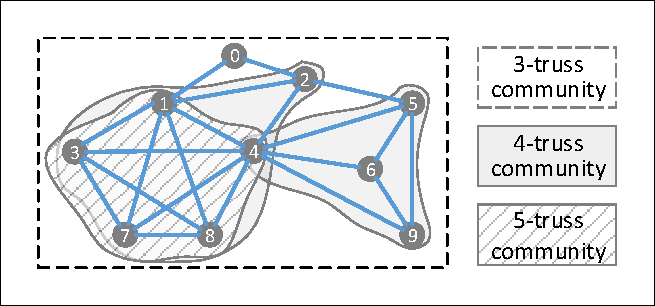
\includegraphics[width=\linewidth]{./figures/k-truss.pdf}
    \caption{An example graph for k-truss community}
    \label{fig:example}
\end{figure}

\autoref{fig:example} shows several examples of k-truss communities. The whole example graph is a 3-truss as every edge has support of at least 1. Note that there are 2 separate 4-truss communities in \autoref{fig:example} as they are not triangle connected with each other.

\textbf{\ProbDef{}} The problem of studied in this paper is defined as follows. Given a graph $G(V,E)$, a set of query vertices $Q \in V$, find all truss communities containing $Q$ with maximum $k$, a specific $k$ or any possible $k$. 